\section{Sequences} 

  We have already defined sequences, but we'll add to our vocabulary to describe and classify sequences and series. To make this chapter a bit more self-contained, we redefine sequences and series. 

  \begin{definition}[Sequence]
    
  \end{definition}

  \begin{definition}[Series]
    
  \end{definition} 

  \begin{definition}[Constant Sequence]
    Let $X$ be any set. 
    \begin{enumerate}
      \item $\{a_i\}$ is a \textbf{constant sequence} if $a_i = A$ for all $i$
      \item $\{a_i\}$ is an \textbf{ultimately constant sequence} if $a_i = A$ for all $i > N$ for some $N \in \mathbb{N}$. If $A = 0$, then $\{a_i\}$ is \textbf{finary}.
    \end{enumerate}
  \end{definition}

  Depending on the structure of $X$, we can further classify series. 

  \begin{definition}[Bounded Sequences]
    Let $(V, ||\cdot||)$ be a normed vector space. $\{a_i\}$ is \textbf{bounded} if there exists $M$ such that $|x_n| < M$ for all $n \in \mathbb{N}$. 
  \end{definition}

  \begin{definition}[Monotonic Sequences]
    Let $X$ be an ordered set. $\{x_n\}$ is 
    \begin{enumerate}
      \item \textbf{increasing} if $x_{n+1} > x_n$ for all $n$.
      \item \textbf{decreasing} if $x_{n+1} < x_n$ for all $n$.
      \item \textbf{nondecreasing} if $x_{n+1} \geq x_n$ for all $n$.
      \item \textbf{nonincreasing} if $x_{n+1} \leq x_n$ for all $n$.
    \end{enumerate}
    Sequences of these types are called \textbf{monotonic}. 
  \end{definition}

\subsection{Convergent Sequences}

  \begin{definition}[Limit of a Sequence]
    A number $A \in \mathbb{R}$ is called the \textbf{limit of the sequence} $\{x_n\}$, written 
    \[ \lim_{n \rightarrow \infty} x_n = A,\]
    if for every neighborhood $U_A$ there exists an index $N$ such that 
    \[x_n \in U_A \text{ for all } n > N\]
    Equivalently, $A$ is the limit of $\{x_n\}$ if for every $\epsilon>0$, there exists an index $N$ such that
    \[ |x_n - A| < \epsilon \text{ for all } n > N\]
    If $A$ is the limit of $\{x_n\}$, then we say that $\{x_n\}$ \textbf{converges} to $A$. If the limit of $\{x_n\}$ is not well defined or finite, then we say that $\{x_n\}$ is \textbf{divergent}. 
  \end{definition}

  The next few theorems help us develop some intuition behind convergence of sequences. This is where the concept of limit points from topology becomes connected to sequences. In here, a limit point of a sequence is a viable candidate for which a sequence converges to. 

  \begin{theorem}
    Let $\{x_n\}$ be a sequence in a metric space $X$. 
    \begin{enumerate}
      \item $\{x_n\}$ converges to $x \in X$ if and only if every neighborhood of $x$ contains $x_n$ for all but finitely many $n$. 
      \item If $\{x_n\}$ converges to $x$, then $x$ is unique. 
      \item If $\{x_n\}$ converges, then $\{x_n\}$ is bounded. 
      \item If $E \subset X$ and $x$ is a limit point of $E$, then there exists a sequence $\{x_n\}$ in $E$ that converges to $x$. 
    \end{enumerate}
  \end{theorem}
  \begin{proof}
    Listed. 
    \begin{enumerate}
      \item ($\implies$) Let $p_n \rightarrow p \in X$. Then, for every $\epsilon > 0$, there exists $N \in \mathbb{N}$ s.t. $d(p, p_n) < \epsilon$ for all $n > N$. Given neighborhood $B_\epsilon (p), x_n \in B_\epsilon (p)$ for all $n > N \implies$ at most $N$ elements are not in $B_\epsilon (p)$. ($\impliedby$) Now for any $\epsilon > 0$, let every $B_\epsilon (p)$ contain all but finitely many $p_n$. Enumerate them $\{x_{n_k}\}_{k=1}^K$, and let 
      \[\alpha = \max \{n_k\}\]
      This means that there exists an $\alpha \in \mathbb{N}$ s.t. $p_n \in B_\epsilon (p)$ for all $n > \alpha$, which implies that $p_n \rightarrow p$. 

      \item Assume $\{p_n\}$ converges to $p, p^\prime \in X$, with $p \neq p^\prime$. Then for all $\epsilon > 0$ there exists $N_1, N_2 \in \mathbb{N}$ s.t. $d(p, p_n) < \epsilon$ for all $n > N_1$ and $d(p^\prime, p_n) < \epsilon$ for all $n > N_2$. This means that there exists a $N = \max\{N_1, N_2\}$ satisfying the above. Since $p \neq p^\prime$, set $\epsilon = d(p, p^\prime) /2$. Then, 
      \[d(p, p_n) < \frac{d(p, p^\prime)}{2} \text{ and } d(p^\prime, p_n) < \frac{d(p, p^\prime)}{2}\]
      which implies that by adding both sides and invoking triangle inequality, we have 
      \[d(p, p^\prime) \leq d(p, p_n) + d(p^\prime, p_n) < d(p, p^\prime)\]
      which is absurd. 

      \item Choose any $\epsilon > 0$. Then from (a), $B_\epsilon (x)$ contains all but finitely many $V = \{x_{n_k}\}_{k=1}^K$. Take 
      \[M = \max \{\epsilon, d(x_{n_1}, x), \ldots, d(x_{n_K}, x)\}\]
      and so $d(x, x_n) < M$ for all $n \in \mathbb{N}$. 

      \item We can explicitly construct one. Let $p \in E^\prime$. Then choose $\epsilon = 1, \frac{1}{2}, \frac{1}{3}, \ldots$ and for every $\epsilon > 0$, $B_\epsilon (p) \cap E \neq \emptyset$. Choose a $p_n$ within this intersection for every $\epsilon = \frac{1}{n}$. Then, we have $\{p_n\}$ contained in $E$. We want to show that this converges to $p$. Take any $\epsilon > 0$, then there exists $N \in \mathbb{N}$ s.t. $0 < \frac{1}{N} < \epsilon$, and for every $n > N$, $\frac{1}{n} < \frac{1}{N} < \epsilon$. Therefore, for every $n > N$, 
      \[p_n \in B_{1/n} (p) \subset B_\epsilon (p)\]
      which means that $p_n \in B_\epsilon (p)$ for all $n > N$, implying that $\lim_{n \rightarrow \infty} p_n = p$. 
    \end{enumerate}
  \end{proof}


  \begin{theorem}[Properties of Limits]
    Given that $\{x_n\}, \{y_n\}$ are numerical sequences with $y_n \neq 0$ for all $n$, and let 
    \[\lim_{n \rightarrow \infty} x_n = A, \;\;\;\;\;\; \lim_{n \rightarrow \infty} y_n = B \neq 0\]
    then, 
    \begin{align*}
        & \lim_{n\rightarrow \infty} (x_n + y_n) = A + B \\
        & \lim_{n \rightarrow \infty} (c x_n) = c A \\
        & \lim_{n \rightarrow \infty} (x_n \cdot y_n) = A \cdot B \\
        & \lim_{n \rightarrow \infty} \frac{x_n}{y_n} = \frac{A}{B}
    \end{align*}
    It immediately follows that the set of all convergent sequences in $\mathbb{R}^\mathbb{N}$ is a subspace of $\mathbb{R}^\mathbb{N}$. 
  \end{theorem}
  \begin{proof}
    Assume that 
    \[\lim_{n \rightarrow \infty} x_n = A \text{ and } \lim_{n \rightarrow \infty} y_n = B \neq 0\]
    This means that for every $\epsilon > 0$, there exists $N_1, N_2 \in \mathbb{N}$ such that
    \begin{align*}
        |x_n - A| &< \epsilon \text{ for all } n > N_1 \\
        |y_n - B| &< \epsilon \text{ for all } n > N_2
    \end{align*}
    Therefore, for a given $\epsilon$, we wish to prove that there exists a $N$ such that for all $n > N$, 
    \begin{align*}
        1. & |(x_n + y_n) - (A+B)| < \epsilon \\
        2. & |c x_n - cA| < \epsilon \\
        3. & |(x_n y_n) - (AB)| < \epsilon \\
        4. & \bigg| \frac{x_n}{y_n} - \frac{A}{B} \bigg| < \epsilon
    \end{align*}
    \begin{enumerate}
      \item By the triangle inequality, we can see that
      \[|(x_n + y_n) - (A+B)| = |x_n - A| + |y_n - B| \]
      Since we can choose the error between $x_n$ and $A$ for $n > N_1$, and $y_n$ and $B$ for $n>N_2$ as small as we want, we set it to $\epsilon/2$. Then, we have
      \[|(x_n + y_n) - (A+B)| = |x_n - A| + |y_n - B| < \frac{\epsilon}{2} + \frac{\epsilon}{2} = \epsilon\]
      for all $n> N = \max\{N_1, N_2\}$. Therefore, for a given $\epsilon$, there exists an $N$ such that 
      \[|(x_n + y_n) - (A+B)| < \epsilon \text{ for all } n > N\]
      \item This proof is easy. For a given $\epsilon$, we choose the error to be $\frac{\epsilon}{c}$.
      \[|x_n - A| < \frac{\epsilon}{c} \text{ for all } n >N_1\]
      Then, there exists natural number $N_1$ such that
      \[|c x_n - c A| < c |x_n - A| =  c \frac{\epsilon}{c} = \epsilon \text{ for all } n > N_1\]
      \item We first observe that since the limit of $\{y_n\}$ exists, it must be bounded by a value, say $B$. That is, 
      \[|y_n| < Y \text{ for all } n \in \mathbb{N}\]
      Then, we see that
      \begin{align*}
          |x_n y_n - AB| & = |(x_n y_n - Ay_n) + (Ay_n - AB)| \\
          & < |x_n y_n - A y_n| + |A y_n - AB| \\
          & = |y_n| |x_n - A| + |A| |y_n - B|
      \end{align*}
      Suppose $\epsilon > 0$ is given. Then, we can set the error bounds freely; there exists $N_1, N_2 \in \mathbb{N}$ such that 
      \begin{align*}
          |x_n - A| < \frac{\epsilon}{2Y} \text{ for all } n > N_1 \\
          |y_n - B| < \frac{\epsilon}{2|A|} \text{ for all } n > N_2
      \end{align*}
      Then, we can see that 
      \[|x_n y_n - AB| \leq |y_n||x_n -A| + |A| |y_n - B| < Y \cdot \frac{\epsilon}{2Y} + |A| \frac{\epsilon}{2|A|} = \epsilon\]
      for all $n> N = \max\{N_1, N_2\}$.
      \item We use the estimate
      \[\bigg| \frac{A}{B} - \frac{x_n}{y_n} \bigg| = \frac{|x_n| |y_n - B| + |y_n||x_n - A|}{y_n^2} \cdot \frac{1}{1 - \delta(y_n)}, \;\;\; \delta(y_n) = \frac{|y_n - B|}{|y_n|}\]
      For a given $\epsilon > 0$, we find natural numbers $N_1, N_2$ such that 
      \begin{align*}
          |x_n - A| & < \min\Big\{ 1, \frac{\epsilon|B|}{8} \Big\} \text{ for all } n > N_1 \\
          |y_n - B| & < \min \Big\{ \frac{|B|}{4}, \frac{\epsilon B^2}{16(|A| + 1)} \Big\} \text{ for all } n > N_2 
      \end{align*}
      From this we can deduce that 
      \[|x_n| = |x_n - A + A| < |x_n - A| + |A| < |A| + 1\]
      and
      \begin{align*}
          |B| & = |y_n + B - y_n| < |y_n| + |B - y_n| \\
          \implies & |y_n| > |B| - |y_n - B| > |B| - \frac{|B|}{4} > \frac{|B|}{2} \\
          \implies & \frac{1}{|y_n|} < \frac{2}{|B|} \\
          \implies & 0 < \delta(y_n) = \frac{|y_n - B|}{|y_n|} < \frac{|B|/4}{|B|/2} = \frac{1}{2} \\
          \implies & 1 - \delta(y_n) > \frac{1}{2}\\
          \implies & 0 < \frac{1}{1 - \delta(y_n)} < 2
      \end{align*}
      So, we can substitute 
      \begin{align*}
          |x_n| \cdot \frac{1}{y_n^2} \cdot |y_n - B| & < (|A| + 1) \cdot \frac{4}{B^2} \cdot \frac{\epsilon \cdot B^2}{16(|A|+1)} = \frac{\epsilon}{4} \\
          \bigg|\frac{1}{y_n} \bigg| \cdot |x_n - A| & < \frac{2}{|B|} \cdot \frac{\epsilon |B|}{8} = \frac{\epsilon}{4} 
      \end{align*}
      into the final equation to get
      \[\bigg| \frac{A}{B} - \frac{x_n}{y_n}\bigg| < \epsilon \text{ for all } n > N= \max\{N_1, N_2\}\]
    \end{enumerate}
  \end{proof}

  \begin{theorem}
    Given convergent sequences $\{x_n\}$ and $\{y_n\}$, if 
    \begin{equation}
      \lim_{n \rightarrow \infty} x_n < \lim_{n \rightarrow \infty} y_n
    \end{equation}
    then there exists an index $N \in \mathbb{N}$ such that $x_n < y_n$ for all $n > N$. 
  \end{theorem}
  \begin{proof}
    Given $x_n \rightarrow x, y_n \rightarrow y$ and $x < y (\in \mathbb{R})$, then for every $\epsilon > 0$, there exists $N_1, N_2 \in \mathbb{N}$ s.t. $d(x, x_n) < \epsilon$ for all $n > N_1$ and $d(y, y_n) < \epsilon$ for all $n > N_2$. Setting $N = \max\{N_1, N_2\}$, we can say the same for all $n > N$. We choose $\epsilon = \frac{y - x}{2} > 0$. Then, there exists $N \in \mathbb{N}$ s.t. $x_n \in (x - \epsilon, x + \epsilon)$ and $y_n \in (y - \epsilon, y + \epsilon)$ for all $n > N$. Therefore, if $a \in (x - \epsilon, x + \epsilon)$ and $b \in (y - \epsilon, y + \epsilon)$, then 
    \[a < \sup B_\epsilon (x) = x + \epsilon = y - \epsilon = \inf B_\epsilon (y) < b\]
    which implies that $x_n < y_n$ for all $n > N$. 
  \end{proof}

  \begin{theorem}[Squeeze Theorem for Sequences]
    Given sequences $\{x_n\}, \{y_n\}, \{z_n\}$ such that 
    \[x_n \leq y_n \leq z_n\]
    for all $n > N$, if $\{x_n\}$ and $\{z_n\}$ both converge to the same limit, then the sequence $\{y_n\}$ also converges to that limit. That is, 
    \[\lim_{n \rightarrow \infty} x_n = \lim_{n \rightarrow \infty} z_n = A \implies \lim_{n \rightarrow \infty} y_n = A\]
  \end{theorem} 
  \begin{proof}
    We first prove that if there exists a $N \in \mathbb{N}$ s.t. $a_n \leq b_n$ for all $n > N$, then $\lim_{n \rightarrow \infty} a_n = a \leq b = \lim_{n \rightarrow \infty} b_n$. Assume this weren't true, that $a > b$. Then for $\epsilon = \frac{a - b}{2} > 0$, there must exist $M \in \mathbb{N}$ s.t. $a_n \in (a - \epsilon, a + \epsilon)$ and $b_n \in (b - \epsilon, b + \epsilon)$ for all $n > M$. But 
    \begin{equation}
      b_n < \sup (b - \epsilon, b + \epsilon) = b + \epsilon = a - \epsilon = \inf (a - \epsilon, a + \epsilon) < a_n
    \end{equation}
    which contradicts $a_n \leq b_n$. Therefore, $a \leq b$. Therefore, we can use this to get 
    \begin{equation}
      A = \lim_{n \rightarrow \infty} x_n \leq \lim_{n \rightarrow \infty} y_n \leq \lim_{n \rightarrow \infty} z_n = A \implies \lim_{n \rightarrow \infty} y_n = A
    \end{equation}
  \end{proof}
  Note that so far, in order to show that a sequence is convergent, we must identify a real number first and then show using the $\epsilon$-$\delta$ definition that it converges. This might be overkill in a case where we just want to prove that a sequence converges, but we don't care what it converges to. 

  Unsurprisingly, we use the fact that the sequence lives in the reals. We can determine convergence by using Cauchy-completeness, which gives us the ``theorem'' (though it is really a fact by construction). 

  \begin{theorem}[Cauchy-Convergence Criterion]
    A cauchy sequence in $\mathbb{R}$ converges. 
  \end{theorem} 

  The second is not so trivial. We take inspiration from the least-upper-bound property. We can't just say that every bounded sequence converges, since this is not true. However, if we have one more assumption, this is strong enough to guarantee convergence. 

  \begin{lemma}[Convergence Criterion for Monotonic Sequences]
    In order for a nondecreasing (nonincreasing) sequence to be convergent, it is necessary and sufficient that it is bounded above (or below). 
  \end{lemma}
  \begin{proof}
    It satisfies to prove the first case, as the second case can be done similarly without much difficulty. Let $x_n \leq x_{n+1}$. Then the set $\{x_n\}$ is bounded above in $\mathbb{R}$, which has the least upper bound property, and so there exists a least upper bound $x$. We claim that the sequence converges to $x$. For every $\epsilon > 0$, since it is least, there exists at least one $x_N \in (x - \epsilon, x)$. By monotonicity, this means that $x_n \in (x - \epsilon, x)$ for all $n \geq N$, and so the sequence converges to $x$. 
  \end{proof}

\subsection{Divergent Sequences}

  Note that while a convergent sequence can be visualized quite easily by the Cauchy convergence criterion, there are many way in which a sequence can be divergent. 
  \begin{enumerate}
    \item Increasing/decreasing indefinitely
    \item Oscillating between two constant values
    \item Oscillating between a value tending to $+\infty$ and a value tending to $-\infty$
    \item Many other classes of divergence
  \end{enumerate}

  \begin{definition}[Sequence Tending to Infinity]
    The sequence $\{x_n\}$ \textbf{tends to positive infinity} if for each number $c$ there exists $N \in \mathbb{N}$ such that $x_n > c$ for all $n > N$. It is denoted 
    \[x_n \rightarrow + \infty \text{ or } \lim_{n \rightarrow \infty} x_n = + \infty\]
    We define sequences that \textbf{tend to negative infinity} similarly. And $\{x_n\}$ \textbf{tends to infinity} if for each $c$ there exists $N \in \mathbb{N}$ such that $|x_n| > c$ for all $n > N$, which is written 
    \[x_n \rightarrow \infty\]
  \end{definition}

  Note that 
  \[x_n \rightarrow +\infty \text{ or } x_n \rightarrow -\infty \implies x_n \rightarrow \infty\]
  but the converse is not necessarily true. The simple example is the sequence $x_n = (-1)^n n$. Also, it is important to know that a sequence may be unbounded and yet not tend to $+\infty$, $-\infty$, or $\infty$. 

  \begin{example}[Unbounded Sequence that Doesn't tend to $\infty$]
    The sequence $x_n = n^{(-1)^n}$ is divergent yet does not tend to positive infinity, negative infinity, nor infinity. 
  \end{example}

\subsection{Subsequences}

  \begin{definition}[Subsequences]
    A \textbf{subsequence} of $\{ a_n\}$ is a sequence $\{a_{\gamma_k}\}$, where $\{\gamma_k\}$ is a strictly increasing infinite subset of $\mathbb{N}$. 
  \end{definition}

  \begin{lemma}
    $\{x_n\}$ converges to $x$ if and only if every subsequence of $\{x_n\}$ converges to $x$. 
  \end{lemma}
  \begin{proof}
    Let $p_n \rightarrow p$. Then, take any subsequence $\{p_{n_k}\}$ of $\{p_n\}$. For any $\epsilon > 0$, there exists a $N \in \mathbb{N}$ s.t. $d(p, p_n) < \epsilon$ for all $n > N$. Since $N$ is finite and the $n_k$'s are unbounded, there must exist a $K \in \mathbb{N}$ s.t. $n_k > N$ if $k > K$. Therefore, given any $\epsilon > 0$, we have proved the existence of a $K \in \mathbb{N}$ s.t. $k > K \implies n_k > N$, which implies by convergence of $p_n$, that 
    \begin{equation}
      d(p_{n_k}, p) < \epsilon
    \end{equation}
    which by definition means that $p_{n_k}$ converges to $p$. Now, for the other direction, given $\{p_n\}$ with every subsequence converging to $p$, we can take the subsequence $\{p_n\}$ itself ($n_k = k$), which converges to $p$. 
  \end{proof}

  \begin{definition}[Partial Limits]
    The \textbf{partial limit} of a sequence $\{x_n\}$ is the limit of any of its subsequence.  
    \begin{center}
        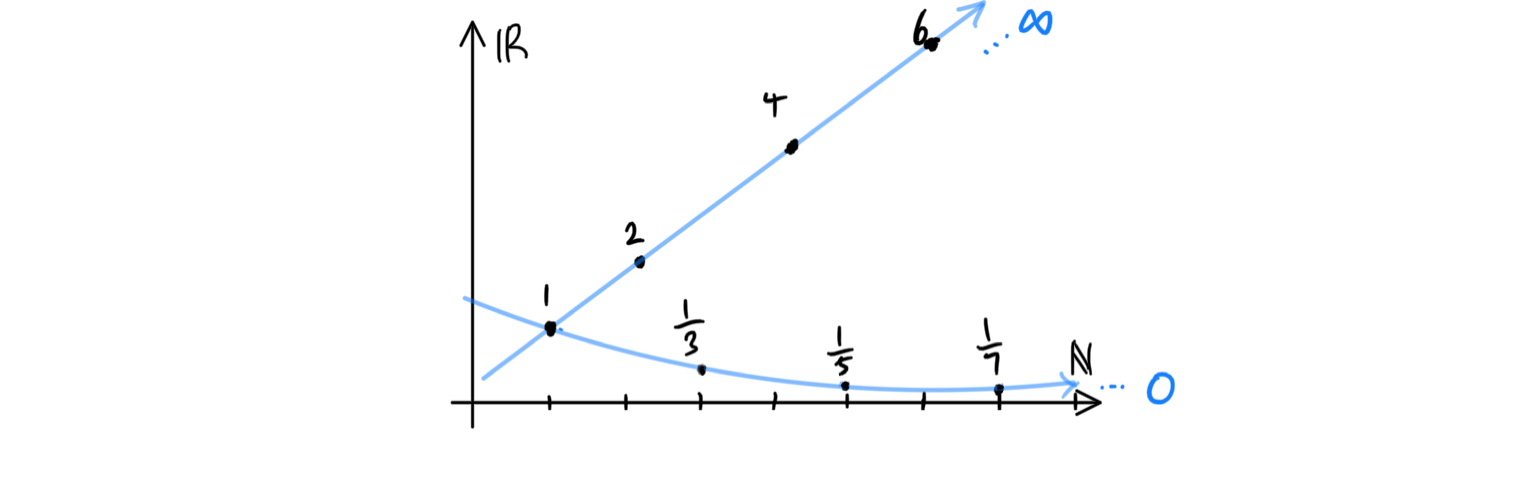
\includegraphics[scale=0.26]{img/Partial_Limit.PNG}
    \end{center}
    Two (out of the many) partial limits of the sequence above is $+\infty$ and $0$. 
  \end{definition}

  \begin{theorem}
    If $\{x_n\}$ is a sequence in a compact metric space $X$, then some subsequence of $\{x_n\}$ converges to a point of $X$.  
  \end{theorem}
  \begin{proof}
    
  \end{proof}

  \begin{corollary}[Bolzano-Weierstrass Theorem]
    Every bounded sequence in $\mathbb{R}^n$ contains a convergent subsequence. 
  \end{corollary} 
  \begin{proof}
    It suffices to prove that there exists a monotonic sequence within a bounded sequence $\{x_n\}$. 
  \end{proof}

  \begin{corollary}
    From each sequence of real numbers there exists either a convergent subsequence or a subsequence tending to infinity. 
  \end{corollary}

  \begin{example}
    We claim that 
    \[\lim_{n\rightarrow \infty} \frac{n}{q^n} = 0 \text{ if } q>1\]
  \end{example}
  \begin{proof}
    Since $x_n = \frac{n}{q^n} \implies x_{n+1} = \frac{n+1}{nq} x_n$ for $n \in \mathbb{N}$. Since 
    \[\lim_{n\rightarrow \infty} \frac{n+1}{nq} = \lim_{n \rightarrow \infty} \bigg(1 + \frac{1}{n}\bigg) \frac{1}{q} = \lim_{n\rightarrow \infty} \bigg( 1 + \frac{1}{n} \bigg) \cdot \lim_{n\rightarrow \infty} \frac{1}{q} = 1 \cdot \frac{1}{q} = \frac{1}{q} < 1\]
    there exists an index $N$ such that $\frac{n+1}{nq} < 1$ for $n>N$. Thus, we have 
    \[x_n > x_{n+1} = x_n \cdot \frac{n+1}{nq} \text{ for } n > N\]
    which means that the sequence will be monotonically decreasing from index $N$ on. The terms of the sequence
    \[x_{N+1} > x_{N+2} > x_{N+3} > \ldots\]
    are positive (bounded below) and are monotonically decreasing, so it must have a limit. 

    Finding the actual limit is easy. Let $x = \lim_{n \rightarrow \infty} x_n$. It follows from the relation $x_{n+1} = \frac{n+1}{nq} x_n$ that
    \[x = \lim_{n\rightarrow \infty} \big(x_{n+1}\big) = \lim_{n \rightarrow \infty} \bigg(\frac{n+1}{nq} x_n \bigg) = \lim_{n \rightarrow \infty} \frac{n+1}{nq} \cdot \lim_{n \rightarrow \infty} x_n = \frac{1}{q} x\]
    which implies that $\big( 1 - \frac{1}{q}\big) = 0 \implies x = 0$.
  \end{proof}

  \begin{example}
    We claim that
    \begin{equation}
      \lim_{n\rightarrow \infty} \sqrt[n]{n} = 1
    \end{equation}
  \end{example}

  \begin{definition}[Inferior, Superior Limits]
    The \textbf{inferior limit} and \textbf{superior limit} of a sequence $\{x_k\}$ are defined as follows, and they can be shown to be the smallest and largest partial limits of the sequence.\footnote{2nd equality should be proven.} That is, 
    \begin{align*}
      \varliminf_{k \rightarrow \infty} x_k & \equiv \lim_{n \rightarrow \infty} \inf_{k \geq n}{x_k} = \min\{ \lim_{r \rightarrow \infty} y_r\}\\
      \varlimsup_{k \rightarrow \infty} x_k & \equiv \lim_{n \rightarrow \infty} \sup_{k \geq n}{x_k} = \max\{ \lim_{r \rightarrow \infty} y_r\}
    \end{align*}
    where $\{y_r\}$ is any subsequence of $\{x_n\}$. Despite the definition, it isn't too difficult to visualize this. For example, take a look at the superior and inferior limits of the divergent sequence below.
    \begin{center}
      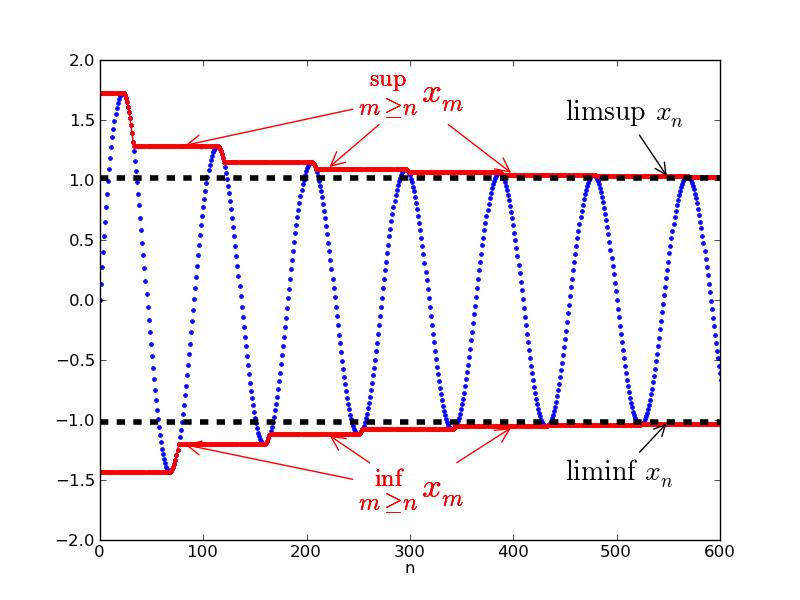
\includegraphics[scale=0.5]{img/Lim_sup_example.png}
    \end{center}
    In order to find the superior limit, we first look the whole sequence in $\mathbb{N}$ and find the supremum. We now "decrease" our domain from $\mathbb{N}$ to $\{2, 3, \ldots\}$, then $\{3, 4, \ldots\}$, then $\{4, 5, \ldots\}$ and so on, continuing to label the supremum of the sequence. The limit of this sequence of supremums is the superior limit. Informally, the superior limit tells us what the supremum of the "end terms" of $\{x_n\}$ will be, and similarly for the inferior limit. 

    The second property of superior and inferior limits is that they represent the greatest and least possible partial limit of a sequence. For example, the six red lines marked in the middle (along with infinitely many others) are viable partial limits because one can choose a subsequence such that all of its points after a certain $n$ lie in some $\epsilon$-neighborhood of the limit. 
    \begin{center}
      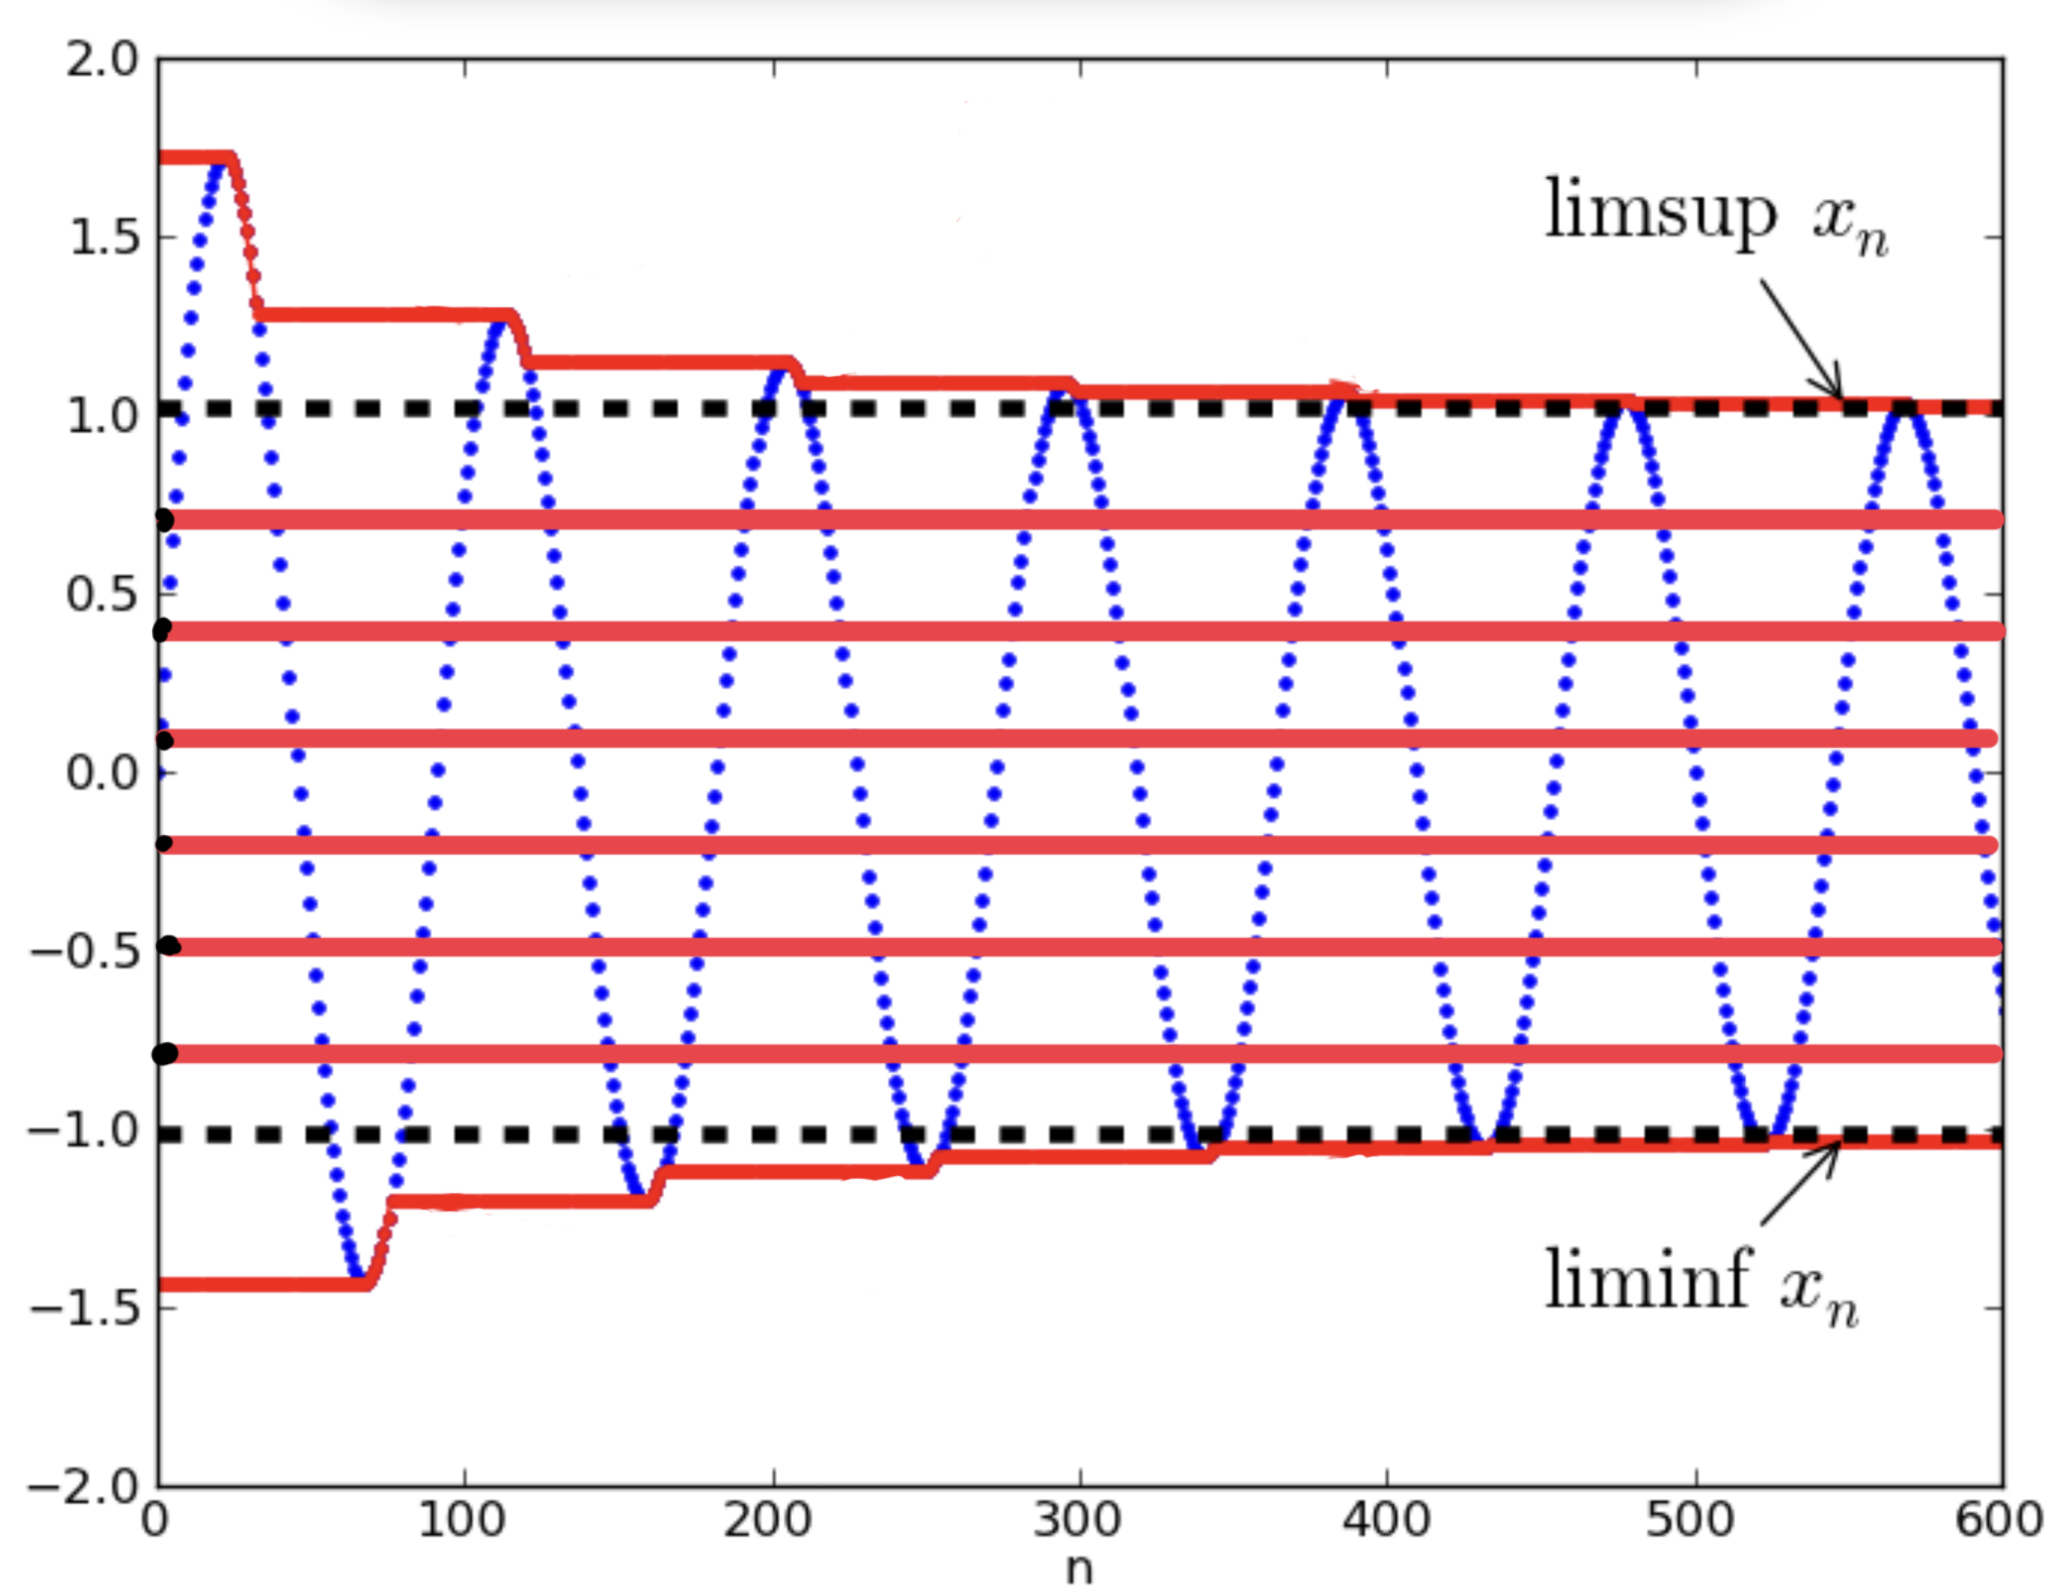
\includegraphics[scale=0.12]{img/Sup_Inf_Limits_as_Limit_Bounds.jpeg}
    \end{center}
    Therefore, the superior and inferior limits represent some sort of "bound" on the sequence in the long run. That is, on the long run, the terms of the sequence $\{x_n\}$ cannot be greater than its superior limit and cannot be less than its inferior limit. With this interpretation, the following theorem should be clear. 
  \end{definition}

  \begin{example}
    Let $s_n = (-1)^n / [1 + (1/n)]$. Then 
    \begin{equation}
      \limsup_{n \rightarrow \infty} s_n = 1, \; \liminf_{n \rightarrow \infty} s_n = -1
    \end{equation}
  \end{example}

  \begin{theorem}
    A sequence has a limit or tends to $\pm \infty$ if and only if its inferior and superior limits are the same. 
  \end{theorem}

  \begin{corollary}
    A sequence converges if and only if every subsequence of it converges. 
  \end{corollary}

  \begin{theorem}
    If $s_n \leq t_n$ for $n \geq N$, where $N$ is fixed, then 
    \begin{align*}
      \liminf_{n \rightarrow \infty} s_n & \leq \liminf_{n \rightarrow \infty} t_n \\
      \limsup_{n \rightarrow \infty} s_n & \leq \liminf_{n \rightarrow \infty} t_n 
    \end{align*}
  \end{theorem}

  \begin{theorem}
    The subsequential limits of a sequence $\{x_n\}$ in a metric space form a closed subset of $X$. 
  \end{theorem}

  \begin{theorem}
    Listed. 
    \begin{enumerate}
      \item If $\overline{E}$ is the closure of a set $E$ in a metric space $X$, then 
      \[\diam{\overline{E}} = \diam{E}\]

      \item If $K_n$ is a sequence of compact sets in $X$ s.t. $K_n \supset K_{n+1}$ for $n \in \mathbb{N}$ and if 
      \[\lim_{n \rightarrow \infty} \diam{K_n} = 0\]
      then $\cap_{n=1}^\infty K_n$ consists of exactly one point. 
    \end{enumerate}
  \end{theorem}
  
\subsection{Convergence Tests for Real Series}

  \begin{definition}[Series over $\mathbb{R}$]
    Given a sequence of real numbers $\{a_n\}$, the \textbf{series} of $\{a_n\}$ is defined
    \begin{equation}
      s = \sum_{k=1}^\infty a_k
    \end{equation}
    The series can be interpreted as the sequence of partial sums $\{s_n\}$, where
    \begin{equation}
      s_n = \sum_{k=1}^n a_k
    \end{equation}
    is the \textbf{$n$th partial term of the series}. Therefore, we can interpret the sum of the series $s$ as the limit of $\{s_n\}$. 
    \begin{equation}
      \lim_{n \rightarrow \infty} s_n = s
    \end{equation}
    If the sequence $\{s_n\}$ converges, the series is \textbf{convergent} and \textbf{divergent} otherwise. 
  \end{definition}

  Since the convergence of a series is equivalent to convergence of its sequence of partial sums, applying the Cauchy convergence criterion to the sequence $\{s_n\}$ leads to the following theorem. 

  \begin{theorem}[Cauchy Convergence Criterion for Series]
    The series $a_1 + \ldots + a_n + \ldots$ converges if and only if for every $\epsilon > 0$ there exists $N \in \mathbb{N}$ such that for all $m \geq n > N$, 
    \begin{equation}
      |a_n + \ldots + a_m| < \epsilon
    \end{equation}
  \end{theorem}

  \begin{definition}[Cauchy Product of Real Series]

  \end{definition}

  \begin{corollary}[nth Term Test]
    A necessary (but not sufficient) condition for convergence of the series $a_1 + \ldots a_n + \ldots$ is that the terms tend to $0$ as $n \rightarrow \infty$. That is, it is necessary that
    \begin{equation}
      \lim_{n\rightarrow \infty} a_n = 0
    \end{equation}
  \end{corollary}
  \begin{proof}
    It suffices to set $m = n$ in the Cauchy convergence criterion. This would mean that for every $\epsilon > 0$ there exists a $N \in \mathbb{N}$ such that 
    \begin{equation}
      |a_n| = |a_n - 0| < \epsilon \text{ for all } n > N
    \end{equation}
    which, by definition, means that $\{a_n\}$ converges to $0$. 
  \end{proof}

  \begin{example}[Geometric Series]
    The series 
    \begin{equation}
      1 + q + q^2 + \ldots + q^n + \ldots
    \end{equation}
    is called the \textbf{geometric series}. 

    Since $|q^n| = |q|^n$, we have $|q^n| \geq 1$ when $|q| \geq 1$. So, if $|q| \geq 1$, the terms $q^n$ does not converge to $0$ and the Cauchy convergence criterion is not met. 

    Now, suppose $|q|<1$. Then, 
    \begin{equation}
      s_n = 1 + q + \ldots + q^{n-1} = \frac{1 - q^n}{1-q}
    \end{equation}
    which implies that
    \begin{equation}
      \lim_{n\rightarrow \infty} s_n = \frac{1}{1-q}
    \end{equation}
    since $\lim_{n\rightarrow \infty} q^n = 0$ if $|q|<1$. This, the series converges to if and only if $|q|<1$, and its sum is $\frac{1}{1-q}$. 
  \end{example}

  \begin{example}[Harmonic Series]
    The series 
    \begin{equation}
      1 + \frac{1}{2} + \frac{1}{3} + \ldots + \frac{1}{n} + \ldots
    \end{equation}
    is called the \textbf{harmonic series}, since each term from the second on is the harmonic mean of the two terms on either side of it. Clearly, 
    \begin{equation}
      \lim_{n \rightarrow \infty} a_n = \lim_{n \rightarrow \infty} \frac{1}{n} = 0
    \end{equation}
    but the sequence of partial sums $s_n$ diverges, and thus the harmonic series diverges. 
  \end{example}

  \begin{definition}[Absolute Convergence]
    The series $\sum_{n=1}^\infty a_n$ is \textbf{absolutely convergent} if the series 
    \[\sum_{n=1}^\infty |a_n|\]
    converges. Clearly, every absolutely convergent series because 
    \[\bigg|\sum_{n=1}^\infty a_n \bigg| \leq \sum_{n=1}^\infty |a_n|\]
  \end{definition}

  \begin{theorem}[Direct Comparison Test]
  Let $\sum_{n=1}^\infty a_n$ and $\sum_{n=1}^\infty b_n$ be 2 series with nonnegative terms. If there exists an index $N \in \mathbb{N}$ such that $a_n \leq b_n$ for all $n >N$, then 
  \begin{align*}
      \sum_{n=1}^\infty b_n \text{ convergent } & \implies \sum_{n=1}^\infty a_n \text{ convergent } \\
      \sum_{n=1}^\infty a_n \text{ divergent } & \implies \sum_{n=1}^\infty b_n \text{ divergent }
  \end{align*}
  \end{theorem}

  \begin{theorem}[Limit Comparison Test]
  Suppose the limit 
  \[\lim_{n\rightarrow \infty} \bigg| \frac{a_{n+1}}{a_n} \bigg| = \alpha\]
  exists for the series $\sum_{n=1}^\infty a_n$. Then, 
  \begin{align*}
      \alpha < 1 & \implies \sum_{n=1}^\infty a_n \text{ converges absolutely} \\
      \alpha > 1 & \implies \sum_{n=1}^\infty a_n \text{ diverges} \\
      \alpha = 1 & \implies \text{ Inconclusive}
  \end{align*}
  \end{theorem}

  \begin{theorem}[Root Test]
  Let $\sum_{n=1}^\infty$ be a given series and 
  \[\alpha = \limsup_{n\rightarrow \infty} \sqrt[n]{|a_n|}\]
  Then, the following are true
  \begin{align*}
      \alpha < 1 & \implies \sum_{n=1}^\infty \text{ converges absolutely} \\
      \alpha > 1 & \implies \sum_{n=1}^\infty \text{ diverges} \\
      \alpha = 1 & \implies \text{ Inconclusive} 
  \end{align*}
  \end{theorem}

  \begin{theorem}[Weierstrass M-test for Absolute Convergence]
  Let $\sum_{n=1}^\infty$ and $\sum_{n=1}^\infty b_n$ be series. Suppose there exists an index $N \in \mathbb{N}$ such that $|a_n| \leq b_n$ for all $n>N$. Then, 
  \[\sum_{n=1}^\infty b_n \text{ converges } \implies \sum_{n=1}^\infty a_n \text{ converges absolutely}\]
  \end{theorem}

  The following theorem, while obvious, has interesting consequences. 

  \begin{theorem}[Cauchy]
  If $a_1 \geq a_2 \geq \ldots \geq 0$, the series $\sum_{n=1}^\infty a_n$ converges if and only if the series 
  \[\sum_{k=0}^\infty 2^k a_{2^k} = a_1 + 2 a_2 + 4a_4 + 8a_8 + \ldots \]
  converges. 
  \end{theorem}
  \begin{proof}
  Letting $A_k = a_1 + a_2 + \ldots + a_k$ and $S_n = a_1 + 2a_2 + \ldots + 2^n a_{2^n}$, it is clear that by adding up the inequalities
  \begin{align*}
      & a_2 \leq a_2 \leq a_1 \\
      & 2a_4 \leq a_3 + a_4 \leq 2a_2 \\
      & 4a_8 \leq a_5 + a_6 + a_7 + a_8 \leq 4a_4 \\
      & \ldots \\
      & 2^n a_{2^{n+1}} \leq a_{2^n + 1} + \ldots + a_{2^{n+1}} \leq 2^n a_{2^n}, 
  \end{align*}
  we get
  \[\frac{1}{2}(S_{n+1} - a_1) \leq A_{2^{n+1}} - a_1 \leq S_n\]
  Since the sequences $\{A_k\}$ and $\{S_k\}$ are nondecreasing, and hence from the inequalities we can conclude that they are either both bounded above (which means that they are both convergent since it is a bounded, nondecreasing series) or both unbounded above (which means that they are both divergent since they are nondecreasing and unbounded). 
  \end{proof}

  \begin{corollary}[p-series Test]
  The series 
  \[\sum_{n=1}^\infty \frac{1}{n^p}\]
  converges for $p>1$ and diverges for $p \leq 1$. 
  \end{corollary}
  \begin{proof}
  Suppose $p\geq 0$. By the previous theorem, the series converges or diverges simultaneously with the series 
  \[\sum_{k=0}^\infty 2^k \frac{1}{(2^k)^p} = \sum_{k=0}^\infty (2^{1-p})^k\]
  which is really just a geometric series. A necessary and sufficient condition for the convergence of this series is that $2^{1-p} < 1$, that is, $p>1$. 

  Now suppose $p \leq 0$. The series is then clearly divergent since all of the terms are larger than $1$. 
  \end{proof}

  We finally conclude by giving a theorem about the convergence of some special sequences. 

  \begin{theorem}
    Some special sequences: 
    \begin{enumerate}
      \item If $p > 0$, then $\lim_{n \rightarrow \infty} \frac{1}{n^p} = 0$. 
      
      \item If $p > 0$, then $\lim_{n \rightarrow \infty} \sqrt[n]{p} = 1$. 

      \item $\lim_{n \rightarrow \infty} \sqrt[n]{n} = 1$. 

      \item If $p > 0$ and $\alpha$ is real, then $\lim_{n \rightarrow \infty} \frac{n^\alpha}{(1 + p)^n} = 0$. 
      
      \item If $|x| < 1$, then $\lim_{n \rightarrow \infty} x^n = 0$. 
    \end{enumerate}
  \end{theorem}

\subsection{Exercises}

  \begin{exercise}[Math 531 Spring 2025, PS4.6]
    Consider the set of all bounded sequences of real numbers. That is, we
    consider sequences $\{x_n\}$ for which
    \begin{equation}
      \sup_{n\in\mathbb{N}} |x_n|
    \end{equation}
    exists. For example, the sequence $\{1,2,3,\ldots\}$ does not belong to the set,
    but the sequence $\{1,-\frac{1}{2},\frac{1}{3},-\frac{1}{4},\ldots\}$ does. Call this set $X$. Endow it with
    a metric:
    \begin{equation}
      d(\{x_n\},\{y_n\}) = \sup_{n\in\mathbb{N}} |x_n - y_n|.
    \end{equation}
    Explain why this is a metric. Make sure to explain why the supremum on
    the right hand side exists.
  \end{exercise}

  \begin{exercise}[Math 531 Spring 2025, PS4.7]
    Consider the metric space $(X,d)$ from the previous problem. Is $\overline{B_1(\{0\})}$
    a compact set? Here, $\{0\}$ is just the sequence of zeros: $\{0,0,0,0,\ldots\}$.
  \end{exercise}
  
  \begin{exercise}
    Prove that convergence of $\{x_n\}$ implies convergence of $\{|x_n|\}$. Is the converse true? 
  \end{exercise}
  \begin{solution}
    If $\{x_n\}$ converges to $x$, then for all $\epsilon > 0$, there exists a $N \in \mathbb{N}$ s.t. $|x_n - x| < \epsilon$ if $n > N$. We use the inequality $\big| |x_n| - |x| \big| \leq |x_n - x|$ to show that then for every $\epsilon > 0$ there exists a $N \in \mathbb{N}$ s.t. 
    \[ \big| |x_n| - |x| \big| \leq |x_n - x| \leq \epsilon \]
    and so $\{|x_n|\}$ converges to $|x|$. 
  \end{solution}

  \begin{exercise}
    Calculate 
    \[\lim_{n \rightarrow \infty} \sqrt{n^2 + n} - n\]
  \end{exercise}
  \begin{solution}
    We can compute  
    \begin{align*}
        \lim_{n \rightarrow \infty} \sqrt{n^2 + n} - n & = \lim_{n \rightarrow \infty} (\sqrt{n^2 + n} - n) \cdot \frac{\sqrt{n^2 + n} + n}{\sqrt{n^2 + n} + n} = \lim_{n \rightarrow \infty} \frac{n}{\sqrt{n^2 + n} + n}
    \end{align*}
    where 
    \[A_n = \frac{n}{\sqrt{n^2 + 2n + 1} + n} \leq \frac{n}{2n + 1} \leq \frac{n}{\sqrt{n^2 + n} + n} \leq \frac{n}{\sqrt{n^2} + n} = \frac{n}{2n} = \frac{1}{2} = C_n\]
    $C_n$ is ultimately constant. It suffices to prove that $A_n$ limits to $\frac{1}{2}$ by showing that 
    \[\frac{n}{2n + 1} = \frac{n/n}{(2n+1)/n} = \frac{1}{2 + \frac{1}{n}}\]
    where $\{\frac{1}{n}\}$ is infinitesimal. 
  \end{solution}

  \begin{exercise}[Rudin 3.3]
    If $s_1 = \sqrt{2}$ and 
    \[s_{n+1} = \sqrt{2 + \sqrt{s_n}}\]
    for $n = 1, 2, \ldots$, prove that $\{s_n\}$ converges and that $s_n < 2$ for $n = 1, 2, \ldots$. 
  \end{exercise}
  \begin{solution}
    We can show that $s_n < 2$ by induction. $s_1 = \sqrt{2} < 2$, so the base case is proved. Now, given that $s_n < 2$, $\sqrt{s_n} < 2 \implies 2 + \sqrt{s_n} < 2 + \sqrt{2} < 4 \implies s_{n+1} = \sqrt{2 + \sqrt{s_n}} < 2$ and we are done. 
  \end{solution}

  \begin{exercise}[Rudin 3.4]

  \end{exercise}

  \begin{exercise}[Rudin 3.5]

  \end{exercise}

  \begin{exercise}[Rudin 3.6]

  \end{exercise}

  \begin{exercise}[Rudin 3.7]

  \end{exercise}

  \begin{exercise}[Rudin 3.8]

  \end{exercise}

  \begin{exercise}[Rudin 3.9]

  \end{exercise}

  \begin{exercise}[Rudin 3.10]

  \end{exercise}

  \begin{exercise}[Rudin 3.11]

  \end{exercise}

